% !TEX project = pdflatex
\documentclass[conference,a4paper]{IEEEtran}

\usepackage{packages}
\input{macros}

\begin{document}

\title{Project in Computer Graphics and Computer Vision (2025/26)\\
       \Large Generating synthetic data in Unreal}

\author{

    \IEEEauthorblockN{Ana Oliveira}
    \IEEEauthorblockA{MEI, PG61510}
    \and
    \IEEEauthorblockN{André Miranda}
    \IEEEauthorblockA{MEI, PG60238}
    \and
    \IEEEauthorblockN{Maria Matos}
    \IEEEauthorblockA{MEI, PG61533}
}

\maketitle

\begin{abstract}

This work presents the generation of a synthetic dataset using Unreal Engine and its evaluation for object detection using a YOLO-based deep learning model. A real-world pen was selected as the target object and reconstructed as a 3D model. Synthetic images were generated by placing the object in simulated environments with different positions and conditions. A real image dataset was also created by capturing photographs of the same object in similar scenarios. Both datasets were annotated using the YOLO format and used to train and evaluate object detection models. The objective is to analyze the effectiveness of synthetic data and its capability to support deep learning models when compared with real-world data.

\end{abstract}

\begin{IEEEkeywords}

Synthetic data generation, Unreal Engine, YOLO object detection, deep learning, computer vision, 3D reconstruction, object detection, dataset generation

\end{IEEEkeywords}

\section{Introduction}

Deep learning-based object detection systems require large amounts of annotated data to achieve reliable performance. However, collecting and manually labeling real images can be time-consuming and expensive. Synthetic data generation provides an alternative approach by allowing the creation of controlled datasets using realistic 3D environments.

In this project, Unreal Engine was used to generate synthetic images of a pen in different simulated scenarios. The generated dataset was compared with a real dataset containing photographs of the same object. Both datasets were tested using a YOLO object detector to evaluate the impact of synthetic data on detection performance.

\section{Real Object and Environment Data Acquisition}

The initial stage of this project consisted of collecting visual information from the real-world object and its surrounding environments. After some consideration between each other, we decided to use a unique pen as the target object for detection (Figure~\ref{fig:pen_image}), which was chosen as the target object for the complete synthetic data generation and object detection pipeline.

A set of images of the physical pen was acquired from different perspectives and orientations in order to capture its visual characteristics, including its shape, dimensions, colors, and surface details. These images served as the main reference for the following stages, particularly for the creation of the 3D model.

\begin{figure}[h]
\centering
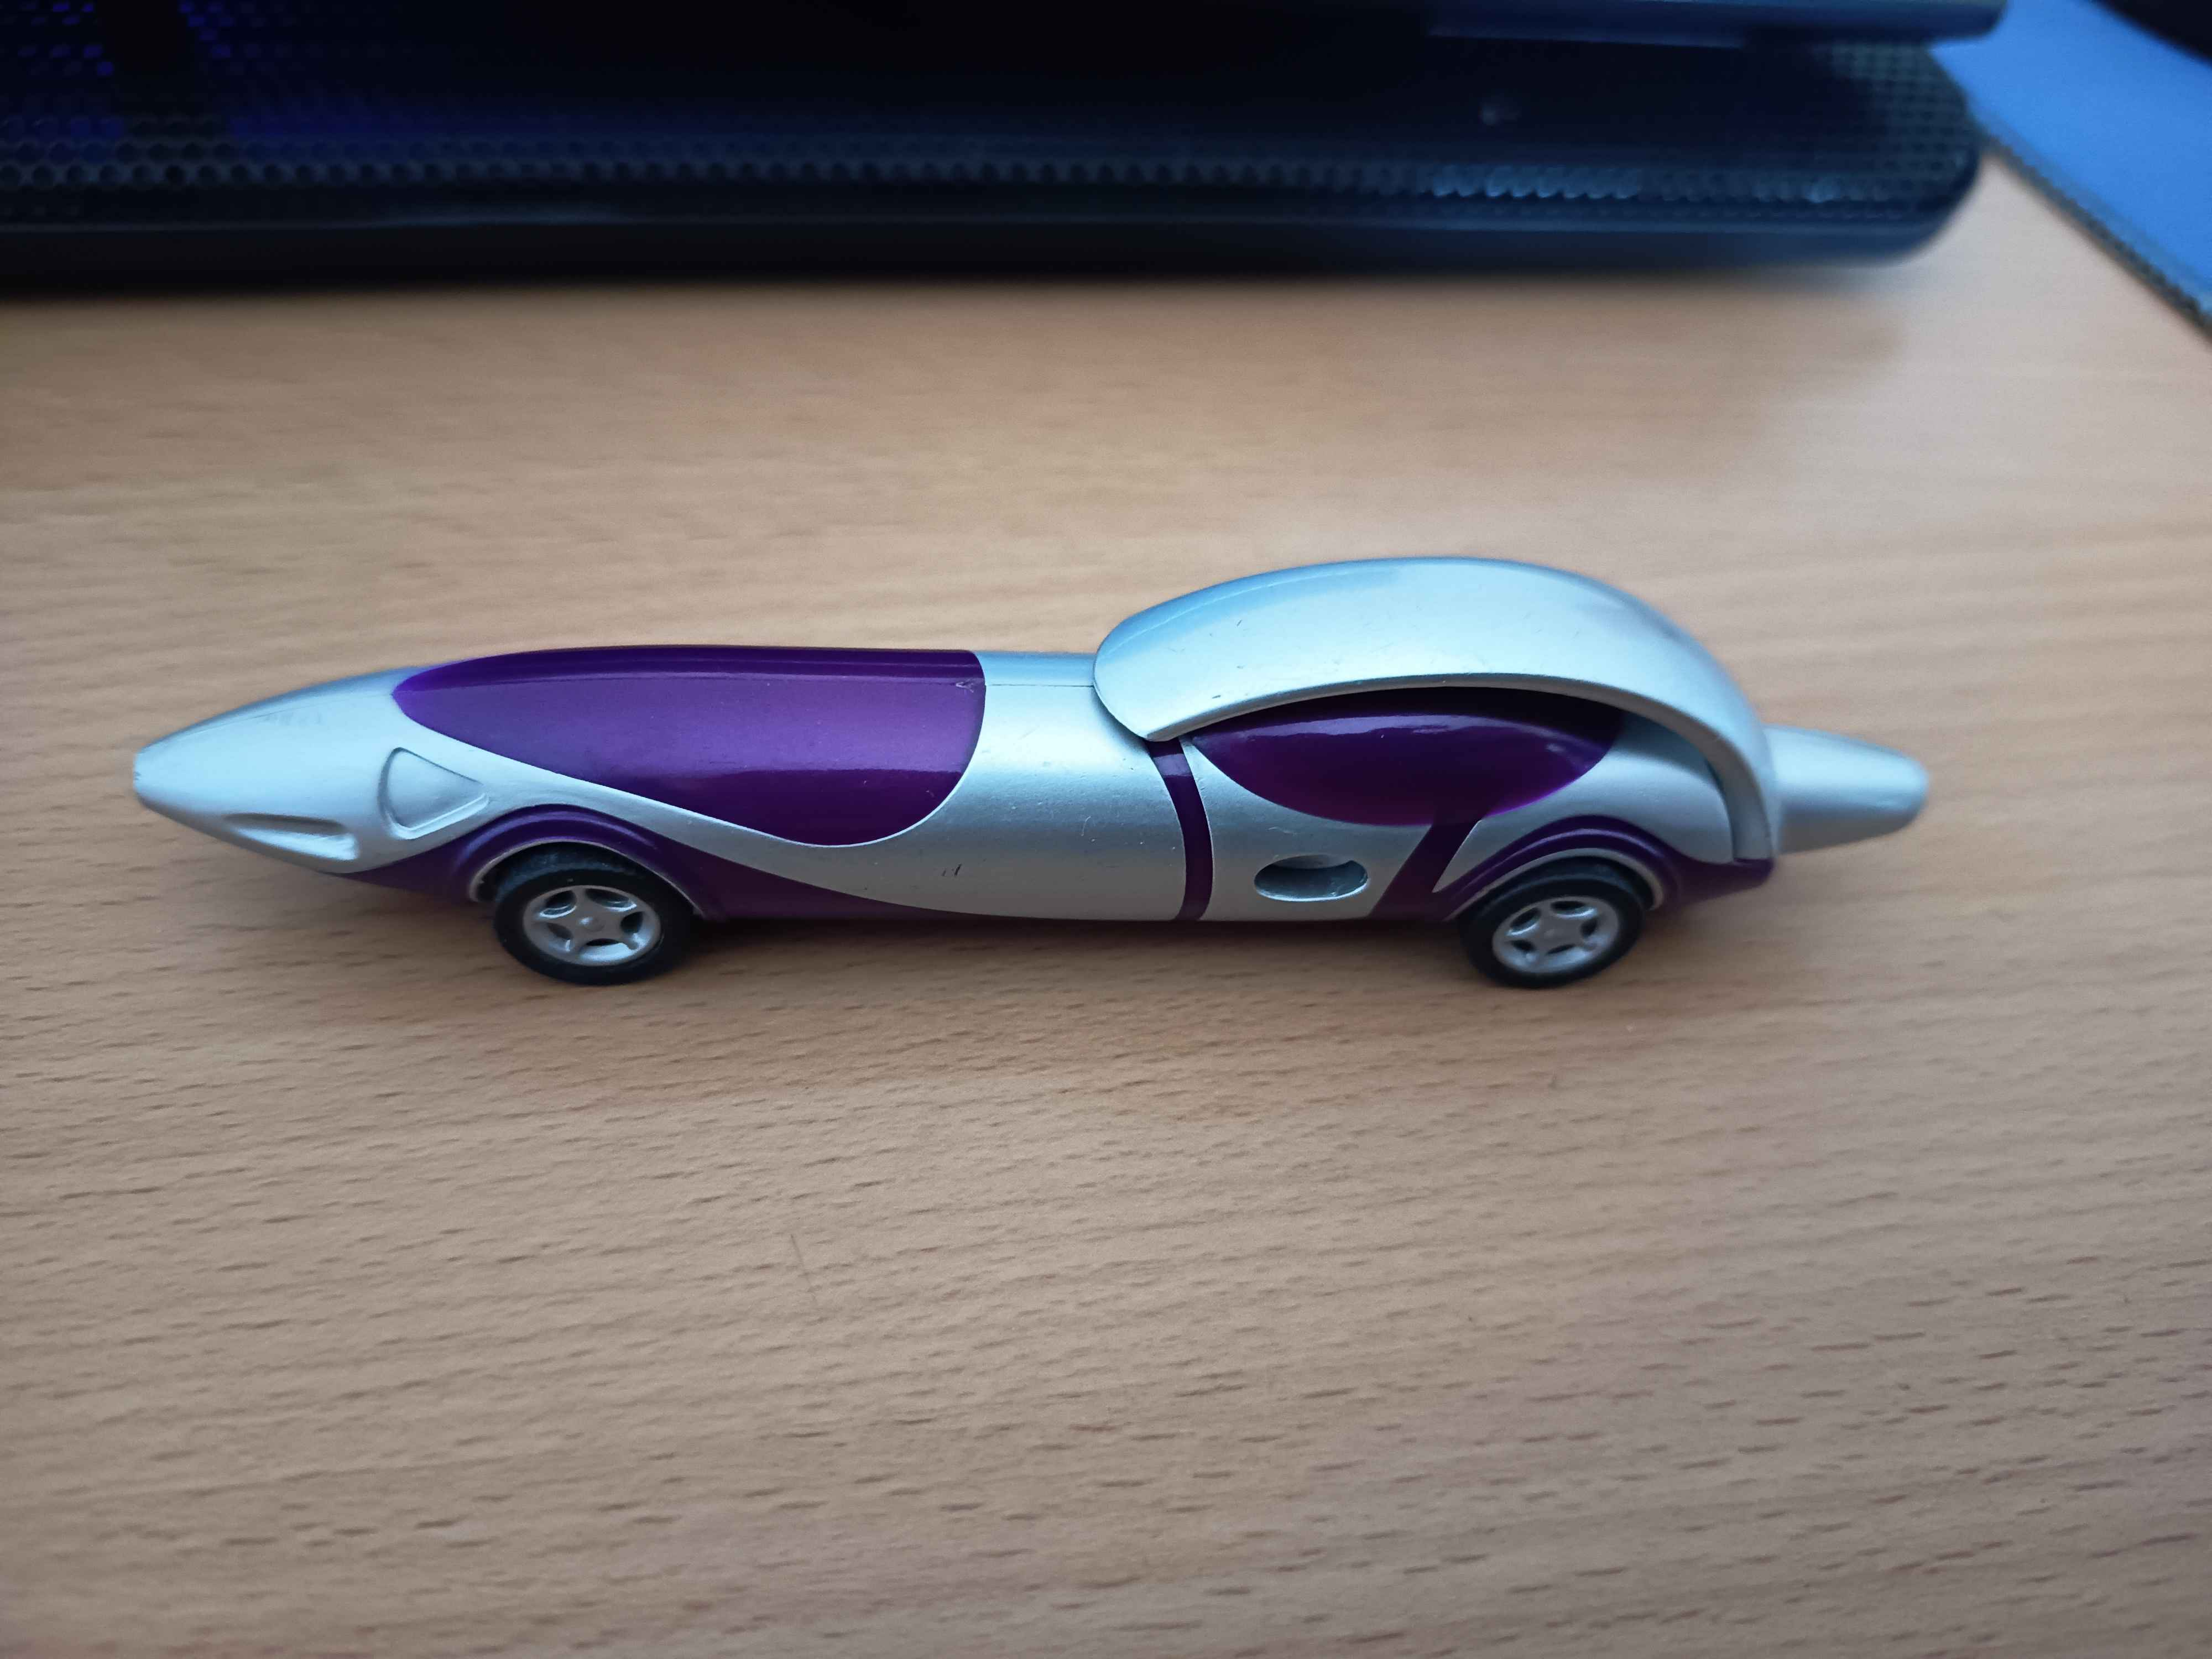
\includegraphics[width=0.45\textwidth]{img/pen_image.jpg}
\caption{Image of the real pen that is used throught the whole project.}
\label{fig:pen_image}
\end{figure}

In addition to the object acquisition, images of possible environments where the pen could naturally appear were also collected (Figure~\ref{fig:real_scenario}). These scenarios provided references for the creation of realistic virtual environments inside Unreal Engine, allowing the generated synthetic images to reproduce conditions closer to real-world situations.

\begin{figure}[h]
\centering
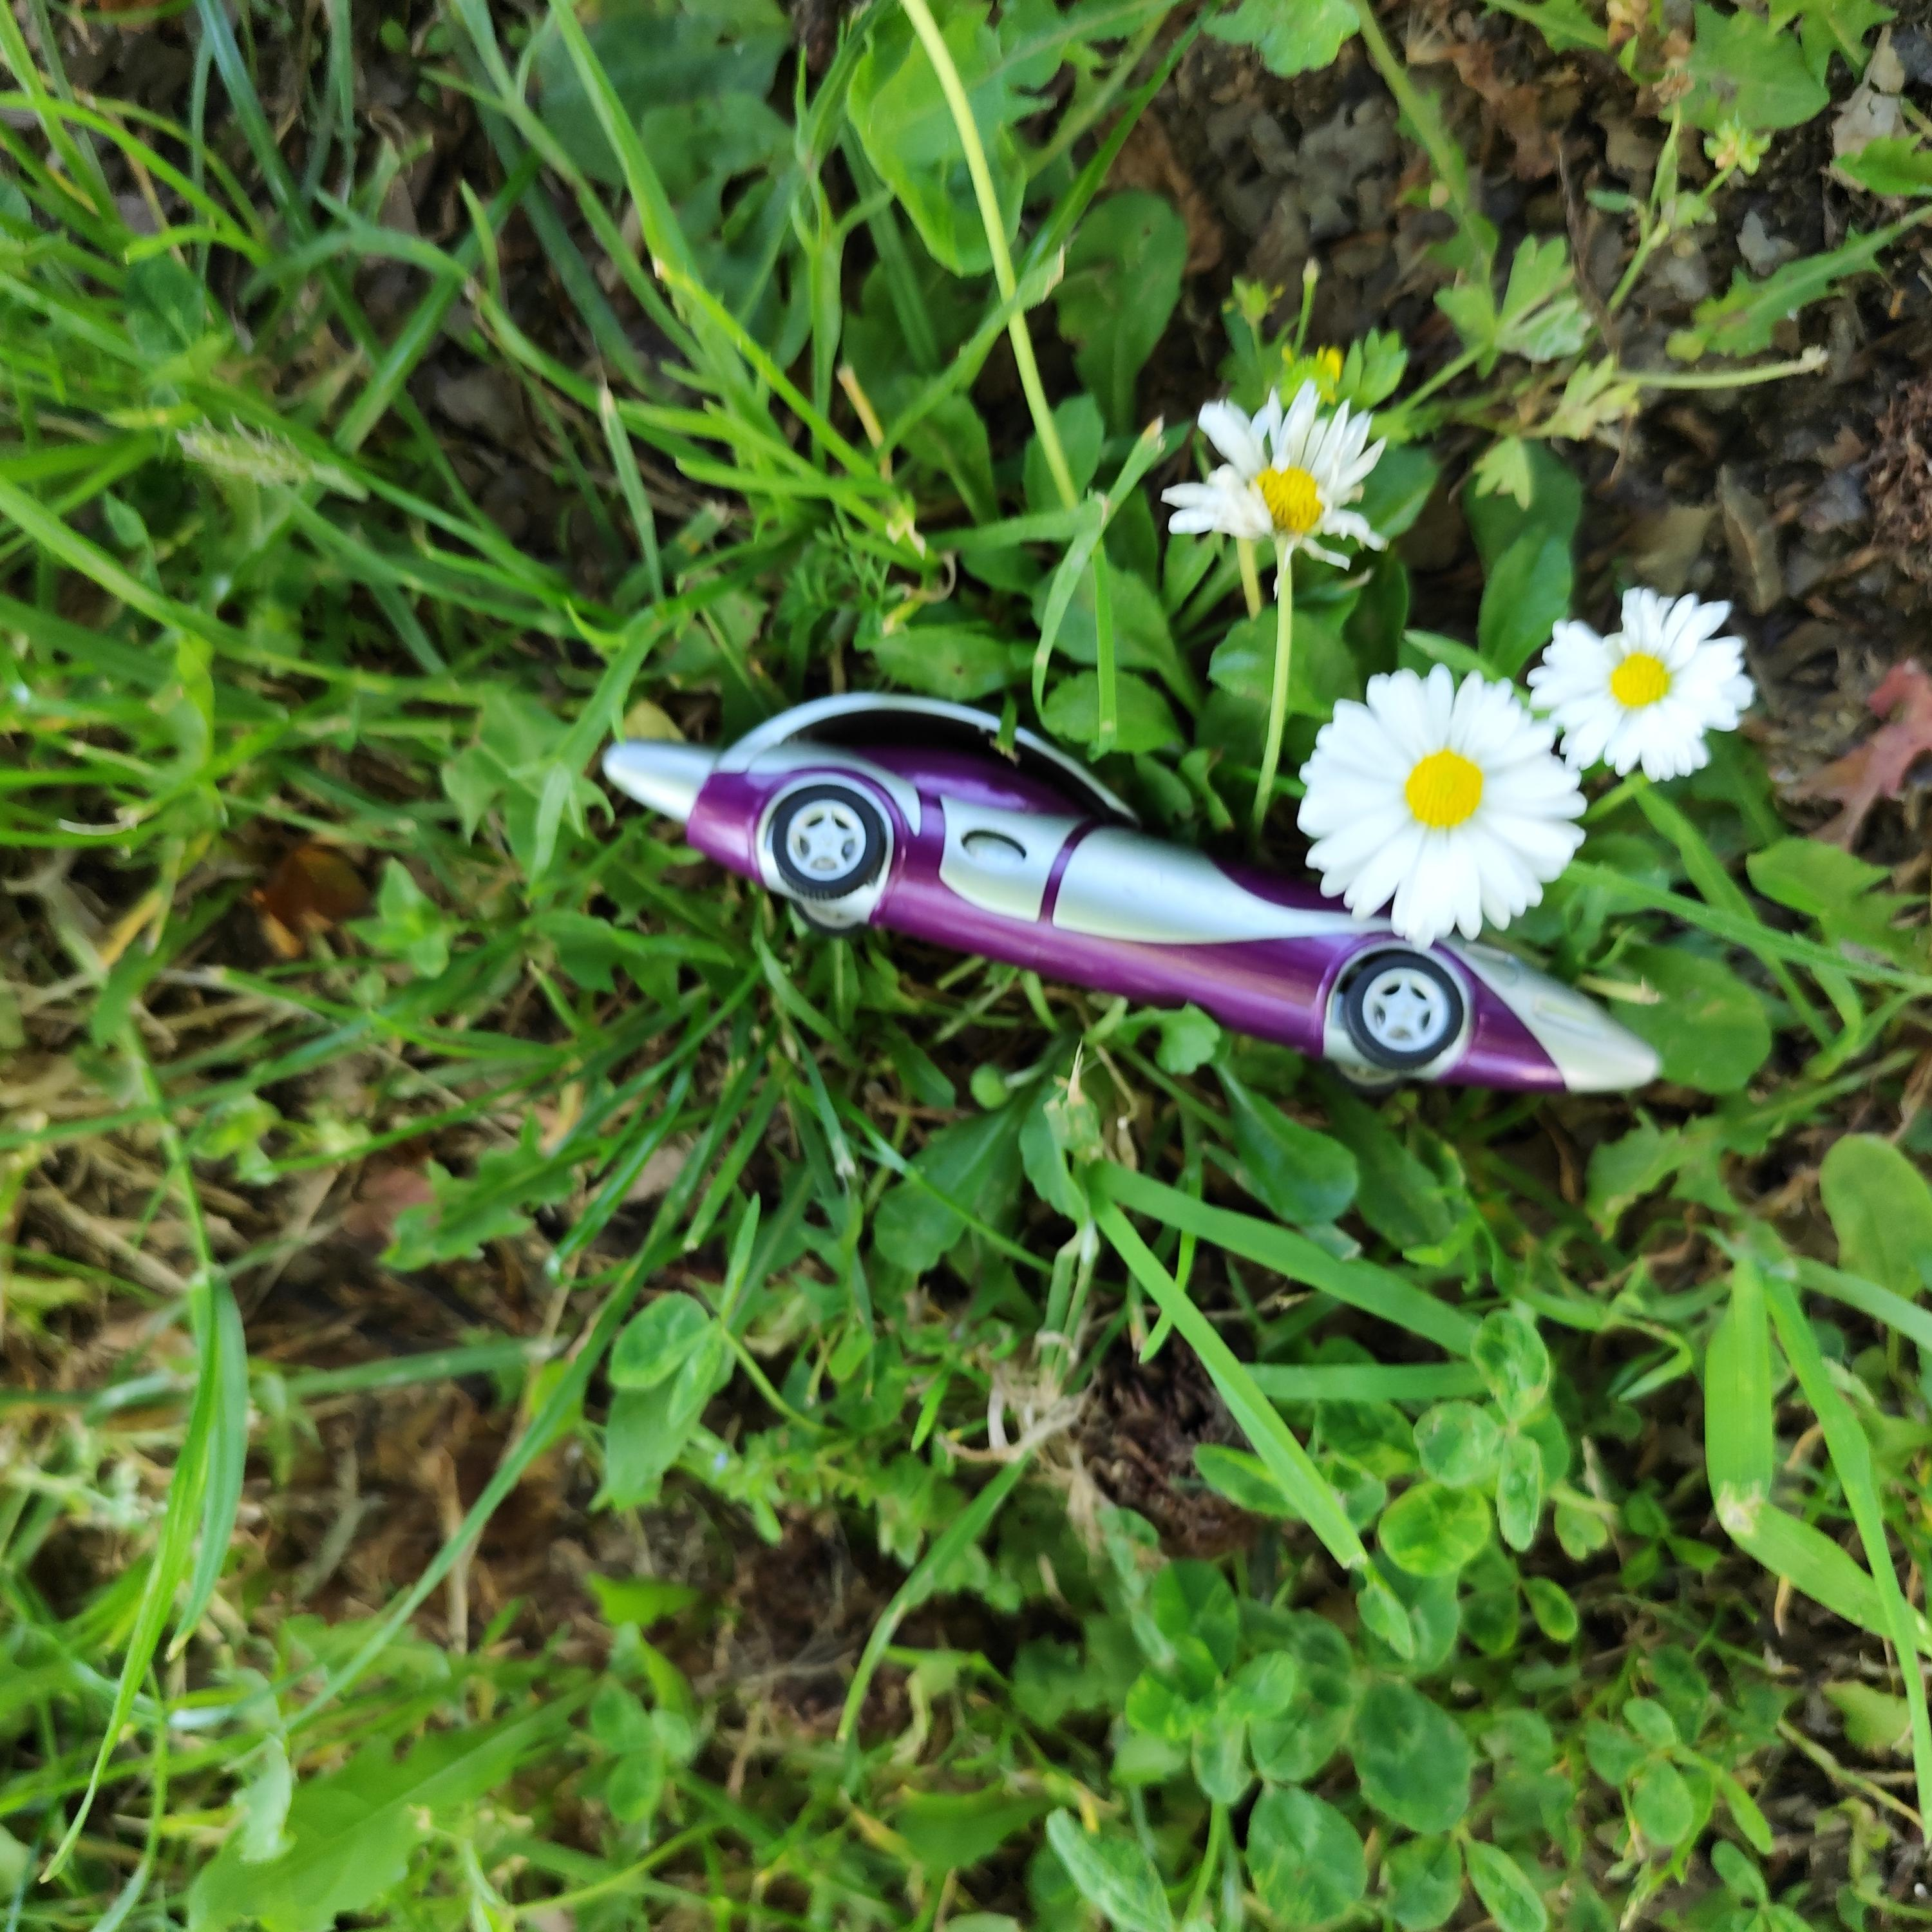
\includegraphics[width=0.30\textwidth]{img/real_scenario.jpg}
\caption{Image of the real pen in a real scenario.}
\label{fig:real_scenario}
\end{figure}

\section{3D Reconstruction of the Object}

After collecting the reference images, the next step consisted of creating a digital representation of the pen. The objective of this stage was to reproduce the physical object as accurately as possible in a 3D environment.

The reconstruction process focused on representing the geometry and visual properties of the real object. Features such as the shape, proportions, and external appearance of the pen were considered to ensure that the generated model maintained similarities with the real object.

At first we attempted to make it from scratch on the Unreal Engine (Figure~\ref{fig:prototype}) but the results achieved deemed to be doable but also too time consuming.

\begin{figure}[h]
\centering
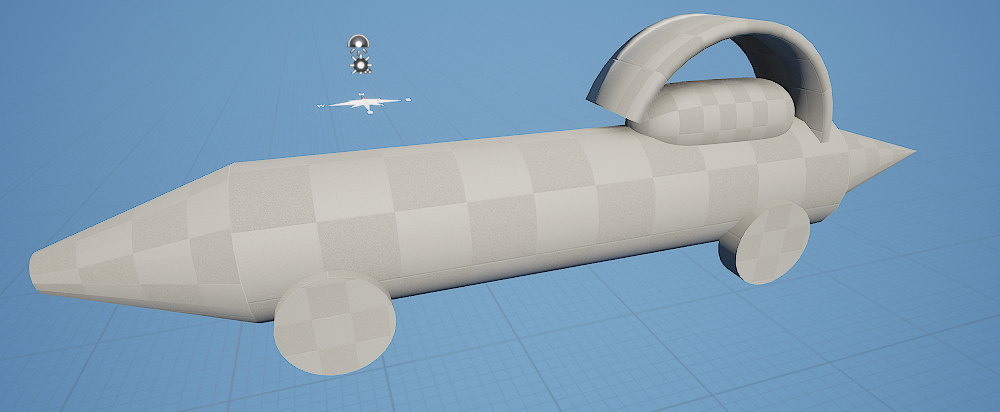
\includegraphics[width=0.45\textwidth]{img/prototype.png}
\caption{Prototype of the synthetic pen made in Unreal Engine.}
\label{fig:prototype}
\end{figure}

By the end of everything, we decided to use application that let us take photos of our pen and then it generated the model in 3D instead of us trying to put the 3D model and the texture of the pen from scratch.

The resulting 3D model was then prepared for integration into Unreal Engine, where it could be placed in different environments and used for synthetic image generation (Figure~\ref{fig:final_result_pen}).

\begin{figure}[h]
\centering
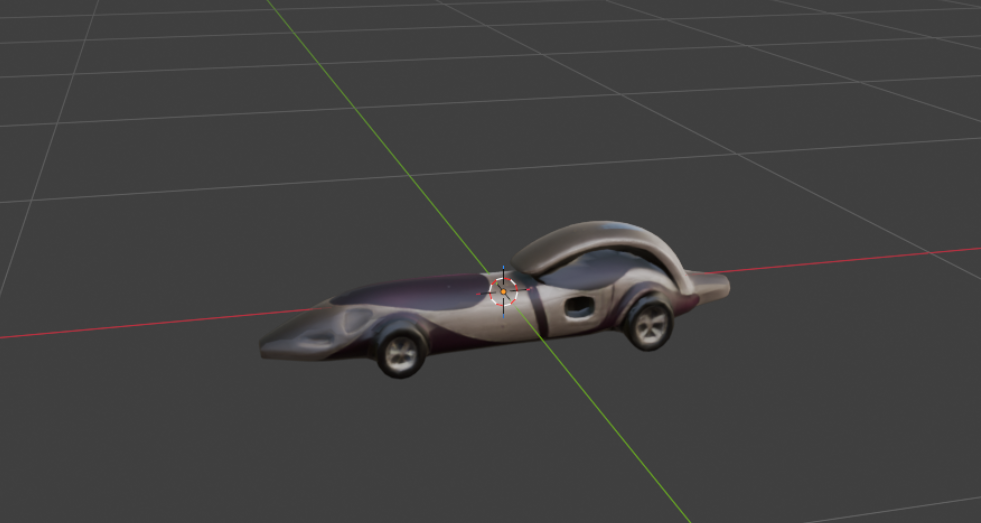
\includegraphics[width=0.45\textwidth]{img/final_result_pen.png}
\caption{Final 3D model of the synthetic pen.}
\label{fig:final_result_pen}
\end{figure}

\section{Unreal Engine Scenario Creation}

After reconstructing the 3D model of the pen, the next stage consisted of creating the virtual environments used for synthetic data generation.

The scenarios were developed in Unreal Engine based on the previously collected images of real environments. The objective was to reproduce realistic conditions where the pen could appear, including similar backgrounds, object positioning, illumination, and camera perspectives.

The reconstructed pen model was placed inside these environments with different orientations and positions. By modifying scene parameters such as lighting, camera angle, and object placement, multiple variations of the same scenario were generated.

This approach would allow the creation of a diverse synthetic dataset while maintaining complete control over the conditions in which the object appears.

The purpose of this stage was to create a dataset containing diverse examples of the pen under different conditions. These images simulate the variability normally present in real-world image acquisition and provide training data for the object detection model.


\begin{figure}[h]
\centering
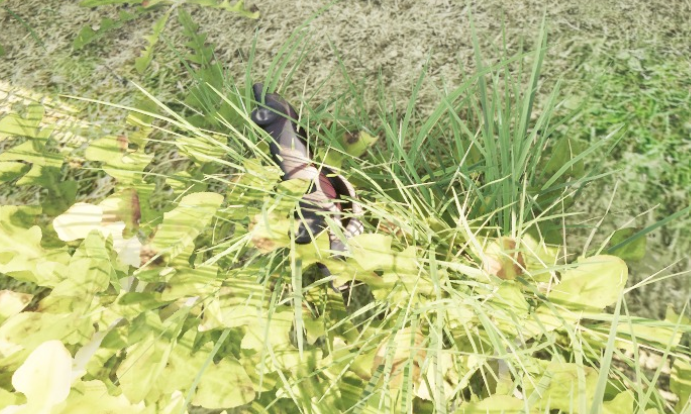
\includegraphics[width=0.45\textwidth]{img/unreal_scene.png}
\caption{Virtual scenario created in Unreal Engine containing the reconstructed pen.}
\label{fig:unreal_scene}
\end{figure}

\section{Real Dataset Creation}

To evaluate the effectiveness of synthetic data, a real image dataset was created containing photographs of the pen in environments similar to the simulated scenarios.

The real dataset provides a reference for evaluating how well the model trained with synthetic images can generalize to real-world conditions. Unlike synthetic images, real images contain natural variations caused by camera limitations, lighting changes, shadows, and background complexity.

The comparison between these datasets allows the analysis of the potential benefits and limitations of synthetic data generation.

\section{Real Dataset Annotation}

The real images acquired from the physical pen require manual annotation before being used for object detection training.

The annotation process was performed using LabelImg, a graphical annotation tool that allows the creation of bounding boxes around objects in images.

For each image, a bounding box was manually placed around the pen and assigned to the corresponding object class. The annotations were exported in YOLO format, generating a text file for each image.

Each YOLO annotation file contains the following information:

\begin{verbatim}
class_id x_center y_center width height
\end{verbatim}

For example:

\begin{verbatim}
15 0.626333 0.527500 0.300000 0.243000
\end{verbatim}

The values are normalized according to the image dimensions, allowing YOLO to process images with different resolutions.

\begin{figure}[h]
\centering
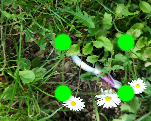
\includegraphics[width=0.45\textwidth]{img/labelimg_annotation.png}
\caption{Bounding box annotation of the pen using LabelImg.}
\label{fig:labelimg}
\end{figure}

\section{Synthetic Dataset Annotation}

After reconstructing the 3D model of the pen, the next stage consisted of creating the synthetic data generation in Unreal Engine. The initial objective of this stage was to fully automate the dataset creation process by developing a script capable of controlling both camera and object movement, allowing the generation of diverse images with automatically exported YOLO annotations.

The intended pipeline would involve moving the pen and camera across different positions and orientations within the scene, ensuring that the object remained within the camera field of view. Each configuration would then be rendered as an image, while a corresponding script would automatically generate YOLO-format annotation files, storing them separately from the images to avoid inconsistencies between data and labels.

However, due to technical limitations in Unreal Engine and time constraints, the full automation of this process could not be achieved. As a result, the dataset generation pipeline was simplified. A limited number of images were manually captured from the created Unreal Engine environments, ensuring variability in object position, camera angle, and lighting conditions.

These images were then incorporated into the synthetic dataset and manually annotated using the LabelImg tool, generating YOLO-compatible bounding box labels for each image (Figure~\ref{fig:labelimg_synthetic}). Although this approach reduced scalability compared to the original plan, it still allowed the creation of a functional synthetic dataset suitable for training and evaluation.

Despite the lack of full automation, the synthetic dataset still preserved important characteristics such as variation in viewpoint, illumination, and background complexity. These factors ensured that the dataset remained useful for evaluating the impact of synthetic data in object detection tasks.

The final synthetic dataset was therefore composed of Unreal Engine-rendered images combined with manually generated YOLO annotations, providing the necessary structure for training the object detection models used in this work.

\begin{figure}[h]
\centering
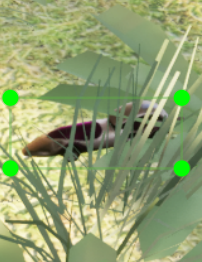
\includegraphics[width=0.45\textwidth]{img/labelimg_annotation_synthetic.png}
\caption{Bounding box annotation of the pen using LabelImg for the synthetic dataset.}
\label{fig:labelimg_synthetic}
\end{figure}



\section{YOLO Object Detection Training}

The object detection models were implemented using the YOLOv8 architecture provided by the Ultralytics library. This framework was selected due to its balance between accuracy and computational efficiency, making it suitable for experiments involving both small and synthetic datasets.

All experiments were initialized using pre-trained weights (yolov8n.pt), enabling transfer learning from large-scale datasets and improving convergence speed during training.

The training pipeline was executed in Python as follows:

\begin{verbatim}
from ultralytics import YOLO

model = YOLO("yolov8n.pt")

model.train(
    data="dataset.yaml",
    epochs=50,
    imgsz=416,
    batch=4
)
\end{verbatim}

Three different experimental setups were defined to evaluate the influence of synthetic data:

\begin{itemize}

\item \textbf{Real dataset training:} The model was trained exclusively using the manually annotated real images of the pen.

\item \textbf{Synthetic dataset training:} The model was trained using images generated from the Unreal Engine environment.

\item \textbf{Combined dataset training (real + synthetic fusion):} Although a unified training experiment combining real and synthetic datasets was initially planned, it was not executed as a single merged training pipeline due to time and implementation constraints. However, a cross-domain evaluation was performed where the synthetic-trained model was tested on real images, providing insight into how synthetic data generalizes to real-world conditions.

\end{itemize}

Each configuration was trained under identical hyperparameters to ensure a fair comparison between datasets. The training process optimized bounding box regression, classification loss, and objectness confidence simultaneously.

The goal of this stage was to evaluate whether synthetic data alone can support robust model training and whether its combination with real data improves overall detection performance.

\section{Model Evaluation}

After the training stage, the performance of the trained YOLOv8 models was evaluated using the validation framework provided by the Ultralytics library. The evaluation was performed automatically during and after training, generating multiple outputs including precision, recall, mean average precision values, confidence curves, confusion matrices, and prediction visualizations.

Instead of manually extracting individual metrics, the trained models were evaluated through the YOLO validation pipeline of this style:

\begin{verbatim}
results = model.val(data="dataset.yaml")
\end{verbatim}

The main evaluation metrics considered were:

\begin{itemize}

    \item \textbf{Precision:} Represents the proportion of correct object detections among all detections generated by the model. Higher precision indicates fewer false positive detections.

    \item \textbf{Recall:} Measures the capability of the model to detect all existing instances of the target object. Higher recall indicates fewer missed detections.

    \item \textbf{mAP0.5:} Represents the Mean Average Precision calculated using an Intersection over Union (IoU) threshold of 0.5. This metric evaluates whether the predicted bounding boxes correctly overlap with the annotated object locations.

    \item \textbf{mAP0.5-0.95:} A stricter evaluation metric that calculates the average precision over multiple IoU thresholds, providing a more demanding evaluation of bounding box localization quality.

\end{itemize}

The validation process was performed for three different scenarios. First, the model trained with real images was evaluated using the real dataset validation split. Second, the model trained only with synthetic images was evaluated using the synthetic dataset validation split. Finally, a cross-domain evaluation was performed, where the synthetic-trained model was evaluated using the real dataset validation split.

This final experiment is particularly relevant because it evaluates whether a model trained exclusively with Unreal Engine generated images can generalize to real-world conditions. The difference between synthetic and real image distributions introduces a domain gap caused by variations in lighting, textures, shadows, background complexity, and camera characteristics.

In addition to numerical evaluation, YOLO automatically generated qualitative results, including predicted bounding boxes, training curves, precision-confidence curves, recall-confidence curves, F1-confidence curves, precision-recall curves, confusion matrices, and label distribution visualizations. These outputs were analysed to better understand the behaviour and limitations of the trained models.

\section{Results}

After completing the training process, the obtained YOLO models were evaluated using the generated metrics and visual outputs provided by the Ultralytics framework. The objective of this evaluation was not only to measure detection accuracy, but also to analyze the capability of synthetic data to transfer knowledge to real-world conditions.

Three evaluation scenarios were considered:

\begin{itemize}
    \item \textbf{Real-to-real evaluation:} The model was trained using real images and evaluated on the real dataset test split. This represents the baseline performance of the detector under the same image domain.
    
    \item \textbf{Synthetic-to-synthetic evaluation:} The model was trained using synthetic Unreal Engine images and evaluated on the synthetic dataset test split. This evaluates whether the generated synthetic data contains enough information for learning the target object.
    
    \item \textbf{Synthetic-to-real evaluation:} The model was trained using synthetic images and evaluated on unseen real images. This experiment evaluates the ability of synthetic data to generalize to real-world conditions.
\end{itemize}


The training process was performed for 100 epochs. During training, the evolution of the main loss components was monitored, including bounding box regression loss (\textit{box loss}), classification loss (\textit{cls loss}), and distribution focal loss (\textit{dfl loss}).

The bounding box loss represents the error associated with object localization. During training, this value progressively decreased and stabilized, indicating that the YOLO model improved its ability to predict the position and size of the pen bounding boxes.

The classification loss also decreased throughout training. Since the dataset contained only one object class, the model did not need to distinguish between different objects, focusing instead on separating the pen from the background.

The distribution focal loss followed the same convergence behaviour, improving the precision of bounding box localization.

\begin{figure}[h]
\centering

\includegraphics[width=0.45\textwidth]{img/results.png}
\caption{Training and validation metrics obtained during YOLO training.}
\label{fig:results}
\end{figure}


\subsection{Performance Comparison Between Evaluation Scenarios}

The final obtained results are summarized below:

\begin{table}[h]
\centering
\caption{YOLO performance comparison between datasets}
\begin{tabular}{c|c|c|c|c}
\textbf{Training} & \textbf{Testing} & \textbf{Precision} & \textbf{Recall} & \textbf{mAP50} \\
\hline

Real & Real Test & 0.999 & 1.000 & 0.995 \\

Synthetic & Synthetic Test & 1.000 & 0.993 & 0.995 \\

Synthetic & Real Test & 0.734 & 0.848 & 0.758 \\

\end{tabular}
\end{table}


The real-to-real experiment achieved the highest overall performance, obtaining:

\begin{itemize}
    \item Precision: 0.999
    \item Recall: 1.000
    \item mAP0.5: 0.995
    \item mAP0.5-0.95: 0.799
\end{itemize}

These results were expected because the training and testing images belong to the same domain. The model was able to learn the appearance of the real pen under similar acquisition conditions, resulting in almost perfect detection performance.


The synthetic-to-synthetic experiment achieved very similar results:

\begin{itemize}
    \item Precision: 1.000
    \item Recall: 0.993
    \item mAP0.5: 0.995
    \item mAP0.5-0.95: 0.733
\end{itemize}

This demonstrates that the synthetic dataset generated in Unreal Engine was sufficiently realistic for YOLO to learn the visual characteristics of the pen. The small difference compared with the real dataset indicates that the generated images contained relevant information regarding object shape, position, and appearance.


However, when the synthetic-trained model was evaluated on real images, performance decreased considerably:

\begin{itemize}
    \item Precision: 0.734
    \item Recall: 0.848
    \item mAP0.5: 0.758
    \item mAP0.5-0.95: 0.294
\end{itemize}

This reduction demonstrates the existence of a domain gap between synthetic and real images. Although the model successfully learned the pen representation from Unreal Engine data, differences between the simulated environment and real-world acquisition affected detection performance.

The main factors contributing to this difference include variations in illumination, shadows, reflections, background complexity, camera characteristics, and object texture appearance. These factors are not completely reproduced in the synthetic environment, making direct transfer more challenging.


\subsection{Dataset Processing and YOLO Training Samples}

Before analysing the numerical metrics, the generated YOLO training samples were inspected to verify the correctness of the dataset preparation.

The training batch visualizations confirm that the images were correctly associated with their corresponding YOLO annotations and that the bounding boxes accurately represented the pen location.

\begin{figure}[h]
\centering

\includegraphics[width=0.35\textwidth]{img/train_batch1.jpg}
\caption{Training samples generated during YOLO training.}
\label{fig:train_batch}
\end{figure}


The validation predictions provide a qualitative analysis of the model behaviour, showing the predicted bounding boxes over unseen images.

\begin{figure}[h]
\centering

\includegraphics[width=0.45\textwidth]{img/val_batch0_pred.jpg}
\caption{YOLO predictions on validation samples.}
\label{fig:val_batch}
\end{figure}


\subsection{Detection Curves}

The confidence curves were analysed to understand the behaviour of the detector under different confidence thresholds.

The precision-confidence curve demonstrates that the detector maintained high precision for the real and synthetic validation scenarios. However, the synthetic-to-real evaluation presented lower confidence reliability due to the increased number of false detections.

The recall-confidence curve shows that the model trained with synthetic images was capable of detecting most objects in synthetic images, but some detections were lost when applied to real images.

The F1-confidence curve demonstrates the balance between precision and recall, with lower performance observed during synthetic-to-real evaluation.

The precision-recall curve confirms the same behaviour, showing that the model maintains strong performance inside the original domain but loses accuracy when transferring between domains.


\begin{figure}[h]
\centering

\includegraphics[width=0.50\textwidth]{img/BoxP_curve.png}
\caption{Precision-confidence curve.}
\end{figure}


\begin{figure}[h]
\centering

\includegraphics[width=0.50\textwidth]{img/BoxR_curve.png}
\caption{Recall-confidence curve.}
\end{figure}


\begin{figure}[h]
\centering

\includegraphics[width=0.45\textwidth]{img/BoxF1_curve.png}
\caption{F1-confidence curve.}
\end{figure}


\begin{figure}[h]
\centering
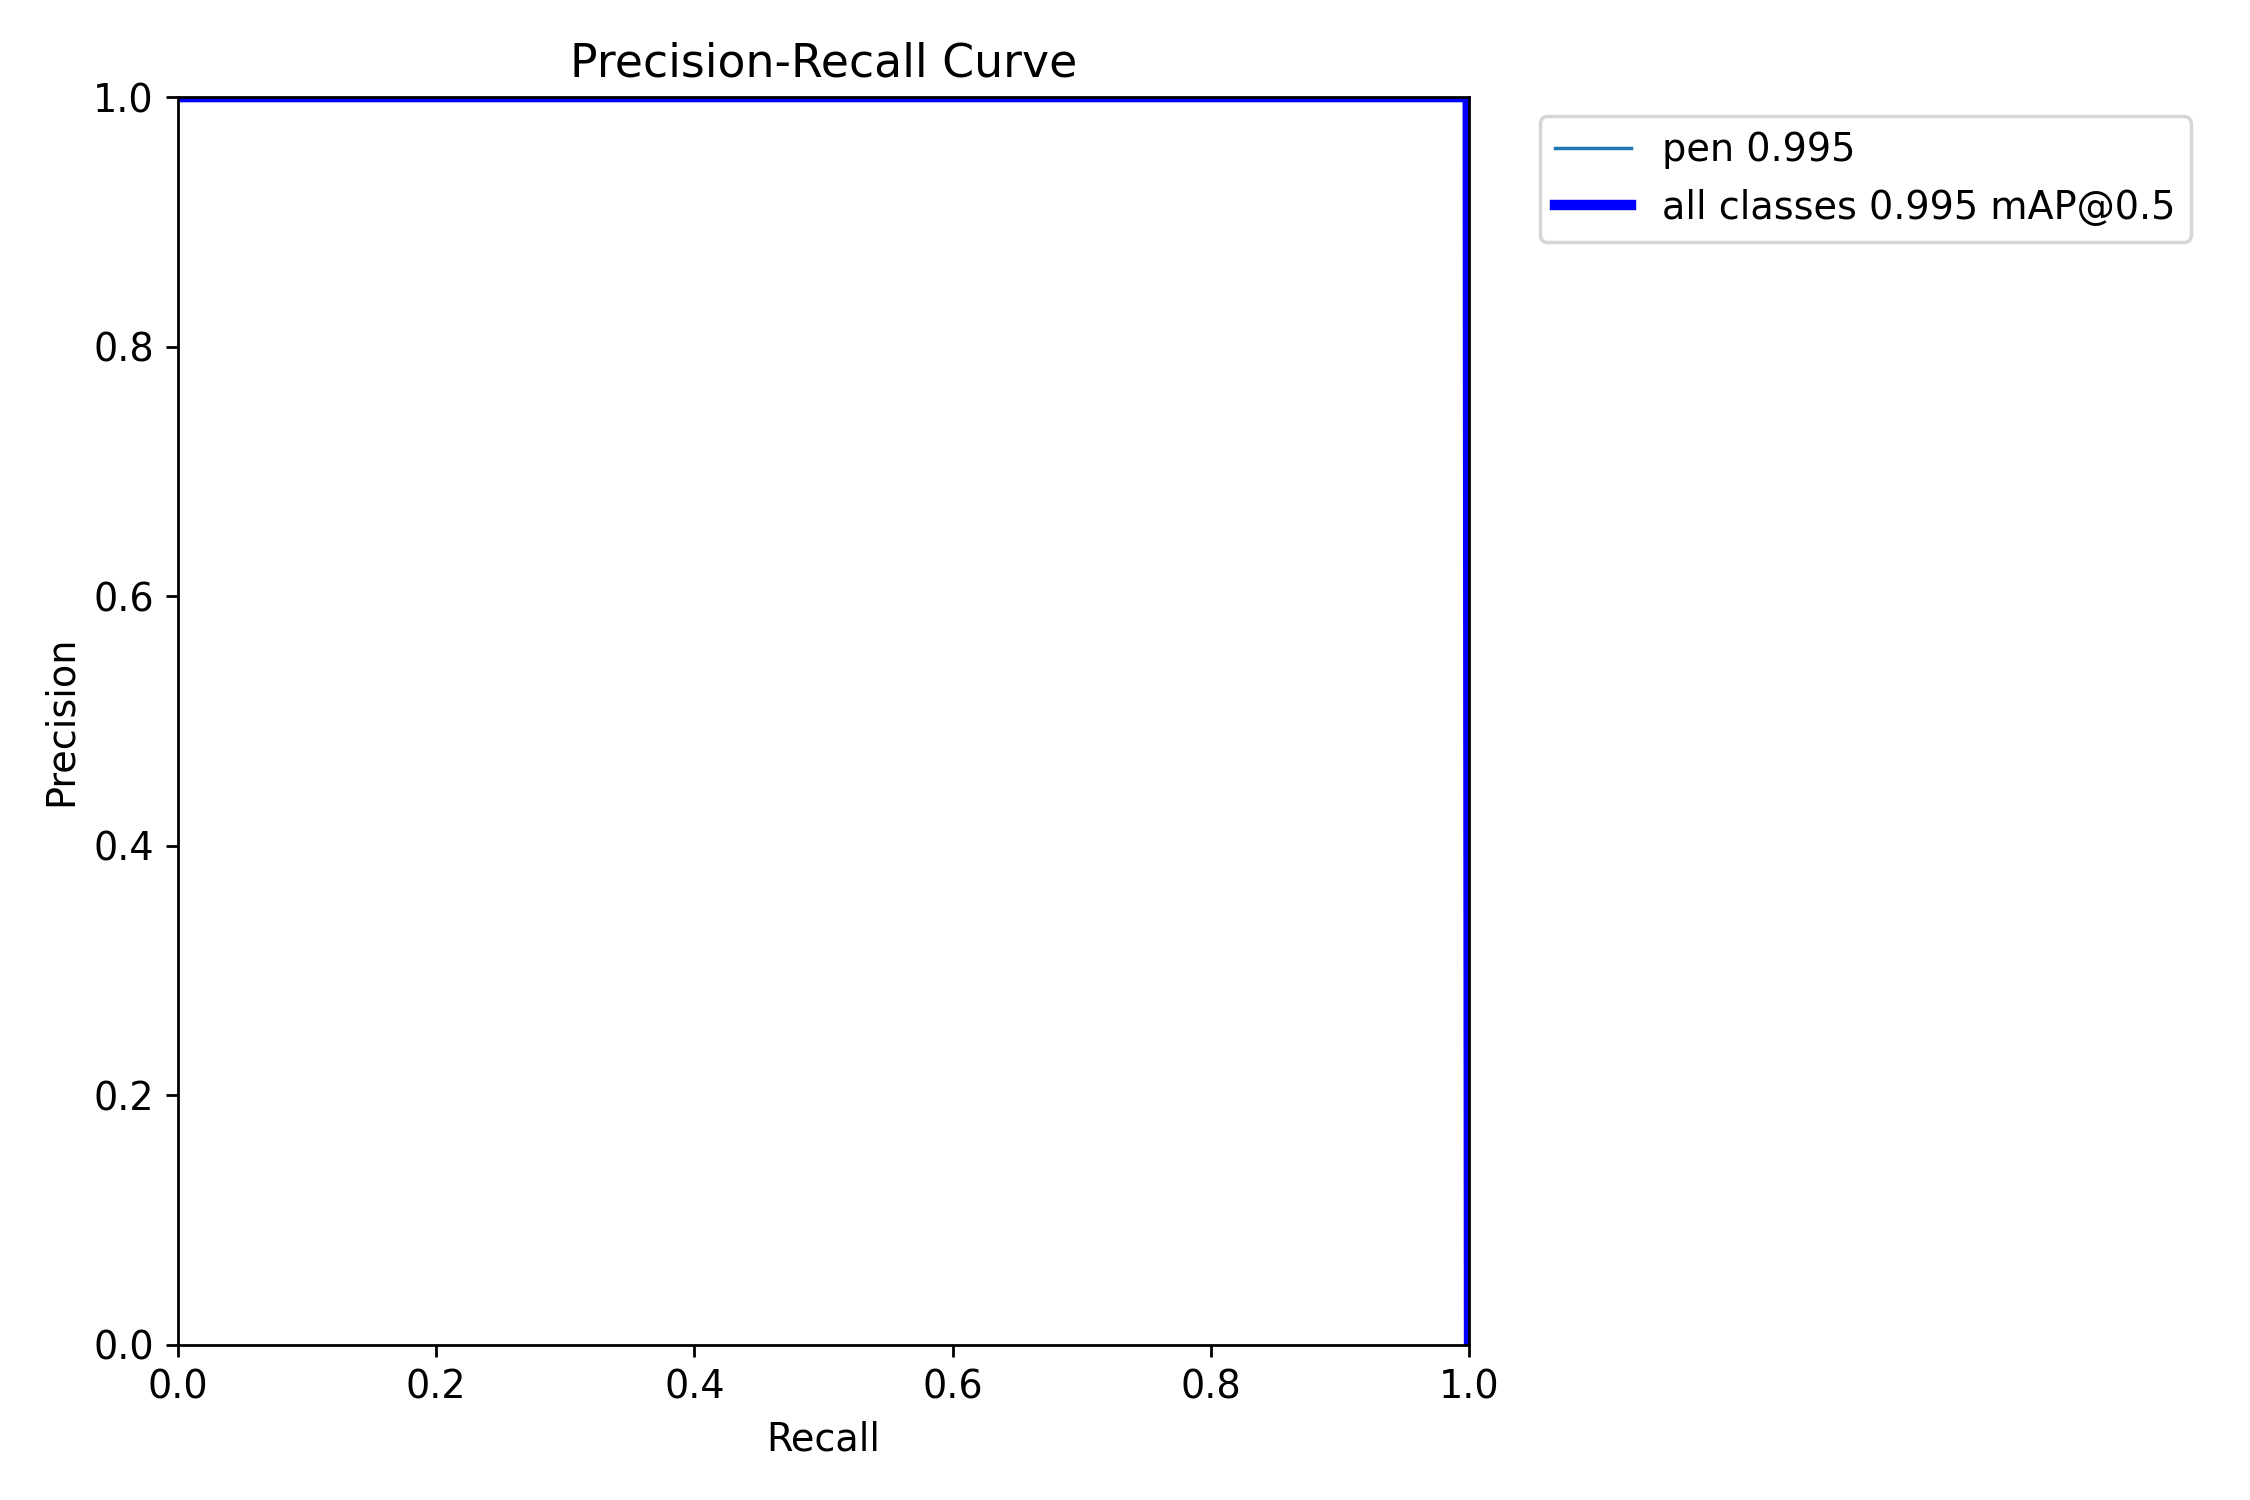
\includegraphics[width=0.45\textwidth]{img/BoxPR_curve.png}
\caption{Precision-recall curve.}
\end{figure}



\subsection{Confusion Matrix Analysis}

The confusion matrices (Figure~\ref{fig:confusion}) were analysed for each experiment.

However, because only one object class was used, the confusion matrices provide limited information. The main classification problem was distinguishing the pen from the background rather than separating multiple object categories.

The matrices mainly confirm the difference in false detections between the same-domain and cross-domain evaluations.

\begin{figure}[h]
\centering

\includegraphics[width=0.45\textwidth]{img/confusion_matrix.png}
\caption{Confusion matrix obtained during evaluation.}
\label{fig:confusion}
\end{figure}



\subsection{Dataset Label Distribution}

The YOLO label distribution was analysed to verify the annotation consistency and ensure that the bounding boxes were correctly generated before training. This analysis provides information about the position, size, and distribution of the annotated objects throughout the dataset. The visualization confirms that the pen annotations were correctly represented in the YOLO format and that the bounding boxes covered the object regions appropriately, reducing the possibility of incorrect labels affecting the training process.

The distribution also provides an overview of the variability present in the dataset, showing differences in object scale and position depending on the image conditions. This variability is important for object detection models, as it allows YOLO to learn different possible appearances and locations of the pen instead of relying on a fixed position or size pattern.

\begin{figure}[h]
\centering

\includegraphics[width=0.40\textwidth]{img/labels.jpg}
\caption{YOLO label distribution.}
\label{fig:labels}
\end{figure}


The obtained results (Figure~\ref{fig:labels}) demonstrate that the complete pipeline successfully created a functional object detection system. The synthetic dataset proved capable of training YOLO inside the simulated environment, but the reduction in performance when applied to real images highlights the importance of reducing the synthetic-to-real domain gap.

\section{Conclusion}

This project presented a complete workflow for the generation of synthetic data and its evaluation for object detection using a YOLO-based deep learning model. Starting from the acquisition of real images of a pen and its surrounding environments, a 3D representation of the object was created and integrated into Unreal Engine to generate realistic simulated scenarios.

The synthetic dataset generated in Unreal Engine enabled controlled variation in object position, camera perspective, illumination, and environmental conditions. In parallel, a real dataset was collected and manually annotated using LabelImg, producing YOLO-compatible bounding box annotations.

Both real and synthetic datasets were used to train and evaluate YOLO-based object detection models under different experimental conditions. The results demonstrated that the model achieved very high performance when evaluated within the same domain, with the real-to-real experiment reaching a precision of 0.999, recall of 1.0, and mAP0.5 of 0.995. Similarly, the synthetic-to-synthetic evaluation also achieved strong performance, confirming that the Unreal Engine-generated dataset contains sufficient visual information for effective learning.

However, when the model trained on synthetic data was evaluated on real images, a significant drop in performance was observed (mAP0.5 = 0.758, mAP@0.5:0.95 = 0.294). This result highlights the presence of a clear domain gap between synthetic and real-world data, mainly caused by differences in lighting, texture realism, background complexity, and camera characteristics.

Despite this limitation, the synthetic dataset still demonstrated meaningful transfer capability, achieving reasonable detection performance even in real-world conditions. This confirms that synthetic data can be a useful resource for training deep learning models, particularly when real data is scarce or expensive to annotate.

The main limitation of this work was the reduced dataset size and the absence of additional object classes, which simplified the detection problem. Future improvements could include generating a larger and more diverse synthetic dataset directly from Unreal Engine, improving automatic annotation generation, and exploring combined training strategies using both real and synthetic data to reduce the domain gap and improve generalization performance.


\begin{thebibliography}{99}

\bibitem{yolov8}
G. Jocher et al.,
``Ultralytics YOLOv8,''
2023. [Online]. Available: \url{https://github.com/ultralytics/ultralytics}

\bibitem{yolo_original}
J. Redmon, S. Divvala, R. Girshick, and A. Farhadi,
``You Only Look Once: Unified, Real-Time Object Detection,''
in \textit{Proceedings of CVPR}, 2016.

\bibitem{unreal}
Epic Games,
``Unreal Engine Documentation,''
[Online]. Available: \url{https://www.unrealengine.com}

\bibitem{pytorch}
PyTorch Contributors,
``PyTorch: An Open Source Machine Learning Library,''
[Online]. Available: \url{https://pytorch.org/}

\bibitem{labelimg}
Tzutalin,
``LabelImg: Graphical Image Annotation Tool,''
[Online]. Available: \url{https://github.com/HumanSignal/labelImg}

\bibitem{opencv}
OpenCV Developers,
``OpenCV Library,''
[Online]. Available: \url{https://opencv.org/}

\bibitem{synthetic_data}
S. Tobin et al.,
``Domain Randomization for Transferring Deep Neural Networks from Simulation to the Real World,''
in \textit{IEEE/RSJ IROS}, 2017.

\end{thebibliography}

\end{document}